% Nome del file: documento.tex
% Percorso: \gl{template}
% Autore: Vault-Tech
% Data creazione: 27.12.2016
% E-mail: vaulttech.swe@gmail.comcom
%
% Diario delle modifiche: interno al file.

\documentclass[a4paper, titlepage]{article}

\usepackage[margin=3cm]{geometry}
\usepackage{../../Stile}
\usepackage{../../Comandi}

\setcounter{secnumdepth}{5}
\setcounter{tocdepth}{5}

\def\NOME{Piano di Qualifica}
\def\VERSIONE{1.0}
\def\DATA{20.01.2016}
\def\REDATTORE{Rudy Berton}
\def\VERIFICATORE{Filippo Tesser \\ & Vassilikì Menarin \\  & Simone Boccato}
\def\RESPONSABILE{Vassilikì Menarin}
\def\USO{Esterno}
\def\DISTRIBUZIONE{\COMMITTENTE \\ & \CARDIN \\ & \PROPONENTE}

\usepackage{graphicx}
\begin{document}
\pagestyle{fancy}	
\pagenumbering{Roman}
\rfoot{Pagina \thepage{} di \pageref{lastromanpage}}

\maketitle

\begin{diario}
	\recap{Approvazione documento}{Vassilikì Menarin}{Responsabile}{20.01.2016}{1.0}
	\recap{Verifica del documento}{Simone Boccato}{Verificatore}{19.01.2016}{0.9}
	\recap{Stesura appendice D}{Rudy Berton}{Analista}{18.01.2016}{0.8}
	\recap{Correzione errori segnalati}{Rudy Berton}{Analista}{16.01.2016}{0.7}
	\recap{Verifica del documento}{Filippo Tesser}{Verificatore}{15.01.2016}{0.6}
	\recap{Stesura appendici A, B e C}{Rudy Berton}{Analista}{11.01.2016}{0.5}
	\recap{Fine stesura Gestione della qualità e stesura sezione Gestione amministrativa della revisione}{Rudy Berton}{Analista}{08.01.2016}{0.4}
	\recap{Inizio stesura Gestione della qualità}{Rudy Berton}{Analista}{05.01.2016}{0.3}
	\recap{Stesura sezione Obiettivi di qualità}{Rudy Berton}{Analista}{03.01.2016}{0.2}
	\recap{Stesura sezione Introduzione}{Rudy Berton}{Analista}{02.01.2016}{0.1}
\end{diario}

\newpage
\tableofcontents

\newpage
\listoffigures

\newpage
\listoftables \label{lastromanpage}

\newpage
\clearpage	
\pagenumbering{arabic}
\rfoot{Pagina \thepage{} di \pageref*{LastPage}}

\hypersetup{linkcolor=blue}
\section{Introduzione}
\subsection{Scopo del documento}
Il presente documento ha lo scopo di descrivere gli obiettivi di qualità, di processo e di prodotto che si intendono perseguire nella realizzazione del progetto, e la descrizione di una strategia di verifica e validazione adottata dal \gl{team} per il raggiungimento di tali obiettivi.

\subsection{Scopo del prodotto}
\SCOPO

\subsection{Glossario}
\GLOSSARIO

\subsection{Riferimenti}
\subsubsection{Riferimenti normativi}
\begin{itemize}
\item \bold{Capitolato d'appalto C5:} Quizzipedia: \gl{software} per la gestione di questionari
\newline \url{http://www.math.unipd.it/~tullio/IS-1/2015/Progetto/C5.pdf};
\item \bold{Norme di progetto: } \NdPdoc;
\item \bold{Analisi dei requisiti: } \ARdoc;
\item \bold{Piano di progetto: } \PdPdoc;
\end{itemize}

\subsubsection{Riferimenti informativi}
\begin{itemize}
\item \bold{Qualità del \gl{software} - Ercole F. Colonese:}
	\newline \url{http://www.colonese.it/00-Manuali_Pubblicatii/06-Qualit%C3%A0Software_v2.pdf}
	\item \bold{La qualità del \gl{software} secondo il modello ISO/IEC9126 - Ercole F. Colonese:} 
	\newline \url{http://www.colonese.it/00-Manuali_Pubblicatii/07-ISO-IEC9126_v2.pdf}
	\item \bold{Metriche del \gl{software} G - Ercole F. Colonese:}
	\newline \url{http://www.colonese.it/00-Manuali_Pubblicatii/08-Metriche%20del%20software_v1.0.pdf};
	\item \bold{The Guide to the \gl{Software} Engineering Body of Knowledge (SWEBOK Guide v3.0) - IEEE Computer Society:} Chapter 10 - \gl{Software} Quality
	\newline \url{http://www.computer.org/web/swebok/;jsessionid=e21ab6073d3593a8523de74bddd2}
\end{itemize}

\newpage
\section{Obiettivi di qualità}
In questa sezione vengono presentate le caratteristiche che definiscono la qualità di prodotto e di processo che il \gl{team} si impegna a soddisfare nella realizzazione del progetto. 
\newline Per ogni caratteristica viene stabilita un'unità di misura che possa quantificarla ed una soglia di accettabilità che il gruppo si prefigge di raggiungere, e possibilmente superare con l'obiettivo di un miglioramento continuo della qualità.

\subsection{Qualità di processo}
Non è possibile distinguere completamente la qualità di processo dalla qualità di prodotto in quanto i risultati dei processi comprendono a loro volta prodotti. Determinare se un processo ha pertanto la capacità di realizzare costantemente prodotti di qualità desiderata non è semplice. 
\newline Per cercare di arginare questa difficoltà vengono stabilite delle caratteristiche da seguire nel tentativo di perseguire una qualità di processo ottimale durante l'applicazione congiunta dei modelli \gl{PDCA} e \gl{CMM}.
\newline Le caratteristiche considerate sono:

\subsubsection{Pianificazione temporale}
Rispettare la pianificazione temporale stabilita nel \doc{Piano di Progetto} è indice di un lavoro che si sta svolgendo nel migliore dei modi; qualora si verifichi un ritardo invece, un campanello d'allarme indicherà che i processi non ancora conclusi non disporranno del grado di qualità atteso per tale scadenza.
\begin{itemize}
\item \bold{Metrica:} l'unità di misura per valutare questa proprietà è la Schedule Variance.
\item \bold{Soglia di accettabilità:} si riterrà accettabile un ritardo al massimo di 4 giorni rispetto a quanto pianificato nel \doc{Piano di Progetto}.
\end{itemize}
Per maggiori dettagli sulla metrica si veda la sezione \hyperref[par:SV]{Schedule Variance}.

\subsubsection{Miglioramento costante}
Per valutare il grado di formalità e ottimizzazione dei processi attuali, con l'obiettivo di apportarne un ulteriore miglioramento alla qualità, viene assunto il modello \gl{CMM} (Capability Maturity Model).
\begin{itemize}
\item \bold{Metrica:} l'unità considerata è la struttura a livelli di cui è rappresentata la Maturità (Maturity) all'interno del modello \gl{CMM}.
\item \bold{Soglia di accettabilità:} si ritiene sufficiente raggiungere il livello 2 (Repeatable), con l'intenzione di migliorare ulteriormente i processi per arrivare anche ad un livello superiore.
\end{itemize}
Per maggiori dettagli sulla metrica si veda la sezione \hyperref[par:cmm]{Capability Maturity Model}. 

\subsubsection{Stima del costo}
Una caratteristica, a lato economico, che stabilisce la qualità dei processi è data dall'aumento dei costi prefissati nel \doc{Piano di Progetto}: qualora un processo non abbia la qualità ottimale richiesta necessita di un miglioramento ulteriore, causando l'aumento dei costi per farlo.
\newline Questo innalzamento del budget non dovrà verificarsi all'interno del progetto se ad ogni processo sarà stata garantita sempre la massima qualità possibile.
\begin{itemize}
\item \bold{Metrica:} l'unità di misura per valutare l'aumento dei costi stabiliti è la Cost Variance.
\item \bold{Soglia di accettabilità:} sarà accettabile quando i costi saranno al massimo superiori del 10\% rispetto a quanto stimato; si cercherà in ogni modo che le stime presentate nel \doc{Piano di Progetto} siano rispettate, senza aumento alcuno.
\end{itemize}
Per maggiori dettagli sulla metrica si veda la sezione \hyperref[par:CV]{Cost Variance}.

\subsection{Qualità di prodotto}
\label{sec:qualprod}
I prodotti che vengono generati nello sviluppo di questo progetto sono principalmente due: i documenti ed il \gl{software}. Vengono pertanto stabiliti gli obiettivi da raggiungere per la diversa tipologia di prodotto considerato.

\subsubsection{Qualità nei documenti}
La stesura dei documenti all'interno di un progetto ricopre un aspetto principale per chiunque collabori nella sua realizzazione come fonte d'informazione, resoconto evolutivo del lavoro svolto, etc. Proprio per la loro importanza i documenti devono presentare un livello di qualità alto, non solo a progetto concluso, ma ad ogni passo dello sviluppo.
\newline Seguendo le caratteristiche riportate in questa sezione il \gl{team} cercherà di redigere della documentazione corretta dal punto di vista grammaticale e contenutistico.

\myparagraph{Correttezza ortografica}
I documenti per essere perfetti in primis devono essere privi di errori grammaticali e ortografici. Sarà effettuata una prima correzione manuale al documento da parte del \italics{Verificatore} ed una successiva verifica automatizzata di supporto attraverso l'uso di uno strumento (\gl{Hunspell}) per garantire una perfetta correttezza ortografica (non è possibile affidarsi unicamente ad un verificatore automatico dal momento che non riesce ad assicurare l'individuazione degli errori al 100\%).  
\begin{itemize}
\item \bold{Metrica:} l'unità di misura è il numero di errori ortografici riscontrati una seconda volta dopo esser stati già segnalati (ma non corretti) durante una precedente verifica del documento, da parte dello strumento automatico e del \italics{Verificatore}.
\item \bold{Soglia di accettabilità:} si accetta di trovare, durante una successiva verifica del documento, al massimo il 5\% degli errori ortografici segnalati durante la verifica precedente (su 100 errori segnalati è accettabile che 5 non siano stati corretti e pertanto risultino segnalati nella verifica successiva).
\end{itemize}
Per maggiori dettagli sulla metrica si veda la sezione \hyperref[par:errort]{Errori ortografici}.

\myparagraph{Leggibilità e comprensibilità}
Un documento poiché risulti utile al proprio fine deve essere leggibile e comprensibile da tutti coloro che possono usufruirne (si consideri come utente tipo un individuo con almeno licenza di istruzione superiore).
\begin{itemize}
\item \bold{Metrica:} l'unità di riferimento è data dall'\gl{Indice Gulpease}.
\item \bold{Soglia di accettabilità:} si riterrà sufficiente un valore superiore a 40 dato dal calcolo dell'\gl{Indice Gulpease}.
\end{itemize}
Per maggiori dettagli sulla metrica si veda la sezione \hyperref[par:IG]{\gl{Indice Gulpease}}.

\myparagraph{Correttezza dei contenuti}
Oltre ad essere esatto dal punto di vista grammaticale un ottimo documento deve presentare del contenuto che sia corretto, coerente e preciso. Sarà compito del \italics{Verificatore} individuare e segnalare gli errori di contenuto presenti all'interno del documento.
\begin{itemize}
\item \bold{Metrica:} il numero di errori concettuali precedentemente segnalati ma non corretti è l'unità di misura che verrà presa in considerazione.
\item \bold{Soglia di accettabilità:} la soglia di accettabilità è inferiore al 5\%; anche se il \gl{team} si prefiggerà il compito di correggere immediatamente qualsiasi errore concettuale segnalato. 
\end{itemize}
Per maggiori dettagli sulla metrica si veda la sezione \hyperref[par:errcon]{Errori concettuali}.

\myparagraph{Adesione alle norme interne}
Ogni documento deve esser redatto secondo le norme definite nel documento \doc{Norme di Progetto}, in tal modo si evitano fraintendimenti sulla lettura da parte dei membri all'interno di un gruppo di sviluppo.
\begin{itemize}
\item \bold{Metrica:} l'unità considerata riguarda il numero di errori  segnalati, ma non corretti, non rispettanti le norme stabilite ad inizio progetto (mancanza del pedice per i vocaboli del \doc{Glossario}, mancanza dei riferimenti ad altri documenti, stile tipografico delle parole sbagliato, etc.). Sarà compito del \italics{Verificatore} individuare tali errori manualmente.
\item \bold{Soglia di accettabilità:} la soglia di accettabilità massima corrisponde al 5\% di errori; si cercherà ad ogni modo di rispettare in modo preciso le norme stabilite.
\end{itemize}
Per maggiori dettagli sulla metrica si veda la sezione \hyperref[par:errfor]{Errori di forma}.

\subsubsection{Qualità nel software}
La qualità di processo, come già detto, influenza direttamente la qualità di un prodotto \gl{software}: se si riesce ad ottenere una buona qualità di processo sarà possibile realizzare un prodotto di qualità ottimale; al contrario un prodotto scarso indicherà che alla base la qualità dei processi non era adeguata.
\newline Il modello che rappresenta in modo ottimale le qualità di un prodotto \gl{software} è lo standard \iso{ISO/IEC 9126}.
\newline Le sue caratteristiche sono:

\myparagraph{Funzionalità}
Tale caratteristica rappresenta la capacità del \gl{software} di fornire le funzioni, espresse ed implicite, necessarie per soddisfare nel modo più completo possibile i requisiti dichiarati nel documento \ARdoc, in modo tale che garantiscano la sicurezza del prodotto, dei suoi componenti e si adegui alle norme.
\begin{itemize}
\item \bold{Metrica:} l'unità di misura per valutare questa caratteristica si basa sul numero di requisiti soddisfatti in modo completo.
\item \bold{Soglia di accettabilità:} la soglia minima di sufficienza è ottenuta qualora almeno tutti i requisiti di natura obbligatoria siano stati soddisfatti.
\end{itemize}
Per maggiori dettagli sulla metrica si veda la sezione \hyperref[par:req]{Requisiti rispettati}.

\newpage
\myparagraph{Affidabilità}
L'affidabilità rappresenta la capacità di un prodotto \gl{software} di mantenere il livello di prestazione in caso di variazioni dell'ambiente circostante. Deve pertanto essere robusto, di facile ripristino e recupero in caso di errori ed aderire alle norme.
\begin{itemize}
\item \bold{Metrica:} la quantità di esecuzioni dell'applicazione avvenute con successo.
\item \bold{Soglia di accettabilità:} la soglia di accettabilità viene raggiunta qualora almeno il 98\% delle esecuzioni produca il risultato atteso.
\end{itemize}
Per maggiori dettagli sulla metrica si veda la sezione \hyperref[par:out]{Output attesi}.

\myparagraph{Usabilità}
È la capacità per un prodotto di essere facilmente comprensibile, apprendibile ed utilizzabile da parte degli utenti finali, in modo tale che soddisfi le aspettative dell'utente e al tempo stesso aderisca alle norme. 
\begin{itemize}
\item \bold{Metrica:} non è facile per questa caratteristica stabilire un'unità di misura oggettiva. Dipende da molti fattori esterni al sistema come le facoltà psicofisiche dell'utente, gli strumenti a disposizione per interagire col sistema, etc.
\item \bold{Soglia di accettabilità:} non esistono metriche obiettive riguardanti l’usabilità. Si cercherà comunque di garantire l'aspetto dell'accessibilità soddisfando gli standard \gl{web} descritti dal \gl{W3C}, portando in questo modo benefici all'usabilità del prodotto.
\end{itemize}
Per maggiori dettagli sulla metrica si veda la sezione \hyperref[par:web]{Validazione \gl{web}}.

\myparagraph{Efficienza}
L'efficienza è la capacità di un prodotto \gl{software} di realizzare le funzioni richieste nel minor tempo possibile e con l'uso minimo di risorse necessarie.
\begin{itemize}
\item \bold{Metrica:} l'unità di misura riguarda il tempo di attesa nella visualizzazione e nel funzionamento dell'applicativo sui diversi dispositivi.
\item \bold{Soglia di accettabilità:} si riterranno accettabili tempi di attesa dell'applicativo non superiori ai 5 secondi durante una transizione eseguita dall'utente.
\end{itemize}
Per maggiori dettagli sulla metrica si vedano le sezioni \hyperref[par:web]{Validazione \gl{web}} e \hyperref[par:greff]{Grado di efficienza}.

\myparagraph{Manutenibilità}
Rappresenta la capacità di un prodotto \gl{software} di essere modificato (senza provocare in seguito effetti indesiderati), corretto in caso di errori o adattato ai cambiamenti dell'ambiente, sempre con l'accortezza che rimanga verificabile.
\begin{itemize}
\item \bold{Metrica:} come unità di misura si considera il numero di correzioni di anomalie non andate a buon fine (che richiedono, cioè, un secondo intervento correttivo) rispetto al numero totale di anomalie risolte.
\item \bold{Soglia di accettabilità:} per rispettare questa qualità si riterranno accettabili valori inferiori al 25\% (su quattro anomalie risolte è accettabile che una sola debba esser risolta una seconda volta).
\end{itemize}
Per maggiori dettagli sulla metrica si veda la sezione \hyperref[par:anins]{Anomalie insufficienti}.

\myparagraph{Portabilità}
L'applicazione dev'essere di facile installazione, esecuzione, adattamento e compatibilità in ambienti \gl{hardware}/\gl{software} diversificati.
\begin{itemize}
\item \bold{Metrica:} numero di \gl{browser} che supportano l'applicazione in modo eccellente, qualsiasi sia il dispositivo utilizzato. 
\item \bold{Soglia di accettabilità:} La soglia di sufficienza per garantire tale caratteristica si avrà quando l'applicativo sarà supportato almeno dalle ultime versioni dei seguenti \gl{browser}: \gl{Google Chrome} , \gl{Mozilla Firefox}, \gl{Safari}, \gl{Opera} ed \gl{Internet Explorer/Edge} (tutti per la versione desktop mentre sono sufficienti i primi tre per dispositivi mobile/tablet).
\end{itemize}
Per maggiori dettagli sulla metrica si veda la sezione \hyperref[par:web]{Validazione \gl{web}}.
\\ 
\newline Le qualità descritte sopra sono quelle interne (proprietà intrinseche del \gl{software}) ed esterne (proprietà che hanno rilevanza solo per l’utente) di un prodotto \gl{software} che il gruppo si prefigge di garantire nello svolgimento dell'applicazione. Queste due categorie vanno ad incidere in una terza tipologia di qualità: la qualità in uso che rappresenta il punto di vista dell'utente finale sulla qualità, una volta che il prodotto sarà completato e in fase di utilizzo. Di questa il \gl{team} non se ne occuperà dal momento che il progetto terminerà prima del rilascio effettivo del \gl{software}.

Per maggiori informazioni sullo standard ISO/IEC 9126 si rimanda all'\hyperref[app:iso]{appendice  C} dedicata.

\newpage
\section{Gestione della qualità: visione generale di strategia}

\subsection{Tecniche di controllo qualità di processo}
La qualità di un processo viene raffinata attraverso un miglioramento continuo grazie al modello \gl{PDCA} (Plan-Do-Check-Act) che in modo incrementale apporta ulteriore qualità a quella precedente. Per rendere effettivo il miglioramento è necessario che ogni attività del modello abbia una scrupolosa pianificazione (possibilmente) proattiva ed un'ottima strategia di verifica che, svolta fin dall'inizio, dovrà permettere una serie di iterazioni all'interno di una determinata fase fino al raggiungimento di un grado di qualità accettabile per poter procedere ad un ulteriore incremento.
\newline La valutazione della qualità di un processo, per poter parlare di un suo possibile miglioramento, dev'essere pertanto quantificata studiando le sue caratteristiche d'interesse; ciò sarà possibile basandosi sul modello \gl{CMM} e sul confronto di performance diverse in momenti differenti.
\newline Un ulteriore indice di valutazione per i processi può esser assunto dalla qualità dei loro prodotti, dal momento che esiste una forte correlazione diretta tra processo e prodotto.

Si vedano le appendici \hyperref[app:PDCA]{\gl{PDCA}} e  \hyperref[app:CMM]{\gl{CMM} - Capability Maturity Model} per maggiori chiarimenti sui modelli adottati.

\subsection{Tecniche di controllo qualità di prodotto}
Il controllo della qualità del prodotto è assicurato da due tipi di processi, quello di verifica e quello di validazione e dal rispetto delle norme.
\begin{itemize}
\item \bold{Verifica:} questo processo si occupa di accertare che l'esecuzione delle attività di processo siano corrette, senza alcun errore. È pertanto un'azione che dev'esser svolta costantemente su ogni attività o risultato che fa progredire il progetto da una \gl{baseline} a quella successiva per poterne assicurare l'assenza di errori.
\\ Il resoconto delle attività di verifica sono descritte nell' \hyperref[app:valtest]{appendice D}.
\\
\item \bold{Validazione:} tale attività viene svolta come atto conclusivo per accertare che il prodotto risultante rispecchi le aspettative sfruttando un metodo sistematico, disciplinato e quantificabile. Sarà pertanto compito del \gl{team} effettuare alla fine dei test per validare il prodotto da consegnare al committente.
\\
\item \bold{Norme:} il prodotto dovrà rispettare le norme e l'uso degli strumenti elencati all'interno del documento \doc{Norme di Progetto}, redatto dal gruppo fin dall'inizio del progetto.
\end{itemize}

\subsection{Responsabilità} 
\label{sec:repo}
La qualità del \gl{software} realizzato è responsabilità di tutti, nessuno escluso. Ogni membro di un gruppo coinvolto in un progetto \gl{software} contribuisce con il proprio lavoro a costruire (positivamente o negativamente) la qualità del prodotto finale e dei processi che ne permettono la realizzazione.
\newline Proprio per questo, qualunque ruolo ricopra, ogni individuo all'interno del \gl{team} deve svolgere le proprie attività con la massima cura al fine di ottenere un grado di qualità alto.
\newline Le responsabilità definite per la qualità a cui ogni ruolo deve adempiere vengono di seguito elencate.
\begin{description}

\item \bold{\italics{Responsabile}}
\begin{itemize}
\item[-]Assicurare che ogni processo sia valutato in maniera oggettiva ed opportunamente migliorato per renderlo sempre più semplice, efficace e conforme alle necessità.
\item[-]Assegnare le responsabilità relative all’assicurazione della qualità a persone indipendenti dallo sviluppo in modo tale che possano verificare, validare e valutare la qualità raggiunta.
\end{itemize}
\ 
\item \bold{\italics{Amministratore}}
\begin{itemize}
\item[-]Assicurare la definizione del processo per la gestione della qualità che ne preveda una fase di pianificazione ed una di controllo.
\item[-]Pianificare la qualità del progetto assicurando la disponibilità delle risorse necessarie sia realizzative che di verifica e validazione.
\item[-] Incentivare nella realizzazione di un processo di verifica sempre più automatizzabile (aumentando il grado d'efficienza).
\item[-]Controllare l’esecuzione di tutte le attività pianificate che assicurino il raggiungimento del livello qualitativo atteso.
\end{itemize}
\ 
\item \bold{\italics{Analista}}
\begin{itemize}
\item[-] Definire e documentare i requisiti funzionali e quelli qualitativi (non funzionali).
\item[-] Deve assicurarsi di aderire agli standard e alle norme riguardanti la documentazione prodotta.
\end{itemize}
\ 
\item \bold{\italics{Progettista}}
\begin{itemize}
\item[-] Indirizzare nelle specifiche tecniche e funzionali anche i requisiti di qualità.
\item[-] Realizzare la progettazione in modo da indirizzare completamente, correttamente ed efficacemente anche i requisiti di qualità.
\item[-] Aderire a tutti gli standard applicabili (standard di programmazione, di documentazione, ...).
\end{itemize}
\ 
\item \bold{\italics{Programmatore}}
\begin{itemize}
\item[-] Sviluppare il codice secondo le norme redatte all'interno del \gl{team} con alto livello di qualità.
\item[-] Aderire a tutti gli standard applicabili (standard di programmazione, di documentazione, ...).
\item[-] Deve fornire test necessari ad eseguire verifiche sulle singole unità prodotte, in modo da verificare il reale livello
qualitativo raggiunto in linea con la criticità e complessità dell’applicazione.
\end{itemize}
\ 
\item \bold{\italics{Verificatore}}
\begin{itemize}
\item[-] Tracciare gli errori rilevati in ciascuna fase del ciclo di sviluppo per poter essere risolti nella stessa fase, verificandone la corretta rimozione.
\item[-] Controllare la corretta esecuzione dei test verificandone lo stato di completamento e stilando un rapporto periodico. 
\item[-] Eseguire le attività di verifica presenti in questo documento valutando processi e prodotti secondo le misure e metriche stabilite.
\end{itemize}

\end{description}
\ 
\newline Per maggiori dettagli circa i ruoli e i compiti assegnati si rimanda al documento delle \doc{Norme di Progetto}.

\subsection{Pianificazione delle scadenze temporali}
Il controllo della qualità deve essere svolto costantemente per garantire la sufficienza dei risultati prodotti, in tal modo sarà possibile progredire nello sviluppo rispettando le scadenze fissate dal committente.
\newline I processi di revisione si dividono in due tipologie: le revisioni formali (esterne) e le revisioni di progresso (interne). Le prime, condotte dal cliente, consentono l'ingresso nella fase successiva di progetto qualora ci sia l'approvazione del prodotto (finale o parziale) dato in ingresso, qualora questo non avvenga si avrà un effetto sanzionatorio. Le seconde invece hanno unicamente una valenza informativa e coinvolgono il cliente; il successo di una tale revisione convalida l’ingresso del fornitore nella fase successiva di progetto.
\newline Le scadenze che il \gl{team} si prefigge di rispettare sono le seguenti:
\begin{itemize}
\item \bold{Revisione dei Requisiti:} 22.01.2016 (revisione formale)
\item \bold{Revisione di Progettazione:} 11.04.2016 (revisione di progresso)
\item \bold{Revisione di Qualifica:} 16.05.2016 (revisione di progresso)
\item \bold{Revisione di Accettazione:} 10.06.2016 (revisione formale)
\end{itemize}
\ 
\newline La pianificazione completa delle attività di progetto è descritta in modo dettagliato nel \PdPdoc.

\subsection{Organizzazione}
All’interno del ciclo di vita è possibile individuare diverse attività principali, descritte nel documento \doc{Piano di Progetto}. All’interno di ciascuna di esse sono pianificati più momenti di verifica, riguardanti le sottoattività svolte, con lo scopo di consolidare i miglioramenti raggiunti all'interno di ogni attività.
\newline L’organizzazione della strategia di verifica viene pertanto suddivisa in base alle sottoattività realizzate durante specifiche attività: per ogni attività sarà disposta una diversa verificazione che vada a controllare sia i processi sia i prodotti ottenuti per mezzo dei primi. Bisogna inoltre prestare attenzione che sottoattività e processi diversi producono a loro volta dei prodotti diversificati; sarà pertanto indispensabile che vengano effettuate distinte procedure di verifica a seconda del processo e prodotto considerato.
\newline Il ruolo all'interno del \gl{team} che ricopre l'incarico di eseguire le verifiche e di segnalare eventuali errori è quello del \italics{Verificatore}, attraverso l'uso degli strumenti messi a disposizione e descritti nel documento \doc{Norme di Progetto}.
\newline Segue l'organizzazione che il \gl{team} ha stabilito per le attività di verifica all'interno del progetto:
\\
\begin{description}
\item[Attività di Analisi requisiti utente]
\ 
\newline In questa prima attività il \gl{team} si trova a produrre molta documentazione pertanto si necessitano tecniche di verifica per garantirne una qualità ottimale. Per far ciò sarà principalmente utilizzata una tecnica di \gl{walkthrough} in cui il \italics{Verificatore} analizzerà ogni documento manualmente per individuare possibili errori al suo interno, anche se sarà affiancato da una verifica automatizzata attraverso alcuni strumenti descritti nelle \doc{Norme di Progetto} (ma non del tutto affidabili).
\newline Attraverso l'uso delle metriche descritte nella sezione \hyperref[sec:metr]{Misure e metriche} sarà possibile valutare quantitativamente la qualità della documentazione per apportarne un miglioramento incrementale fino a raggiungere il grado di qualità atteso. 
\newline Tale verifica della documentazione dev'essere svolta in tutte le attività dell'organizzazione, pertanto anche in quelle seguenti, fino alla conclusione del progetto.
\newline Altra sottoattività fondamentale da svolgere nel contesto iniziale è la corretta individuazione dei requisiti utente con annessi i relativi casi d'uso dal momento che determineranno l'esito finale del progetto. Serve pertanto una scrupolosa sottoattività di verifica da parte del \italics{Verificatore} durante la stesura del documento \doc{Analisi dei Requisiti}.

È possibile visualizzare i valori ottenuti dalla sottoattività di verifica durante questa attività nell'\hyperref[app:valtest]{appendice D}. 
\\
\item[Attività di Raffinamento dei requisiti]
\
\newline Con il superamento della Revisione dei Requisiti, saranno segnalate delle correzioni e dei suggerimenti da parte del committente da apportare ai documenti dati precedentemente in ingresso. 
\newline Si dovrà pertanto produrre un miglioramento alla documentazione ed eventualmente ai requisiti (con i relativi casi d'uso) individuati qualora non soddisfino appieno le aspettative del committente.
\newline Il \italics{Verificatore} avrà in questa occasione il compito anche di controllare che tutte le modifiche siano state svolte in modo corretto secondo le precisazioni date dal committente.
\\
\item[Attività di Progettazione architetturale]
\ 
\newline Viene progettata a questo punto l'architettura del sistema che necessita di una verifica molto precisa poiché si deve garantire che tutti i requisiti utente, stabiliti nell'Attività di Analisi requisiti utente, abbiano una corretta corrispondenza coi moduli progettati.
\\
\item[Attività di Progettazione di dettaglio e codifica]
\ 
\newline In tale attività avviene la progettazione nel dettaglio e la codifica di tutti i requisiti utente obbligatori, e quanti più requisiti
desiderabili e opzionali possibili. 
\newline Sarà ancora necessario che il \italics{Verificatore} tenga traccia dei requisiti svolti dal momento che dovranno risultare soddisfatti tutti quelli indicati durante l'Attività di Analisi requisiti utente (e quelli modificati durante l'Attività di Raffinamento dei requisiti); dovrà inoltre garantire che i prodotti finali rispecchino le caratteristiche definite nella sezione \hyperref[sec:qualprod]{Qualità di prodotto} (siano essi documenti oppure prodotti \gl{software}) attraverso la valutazione di misure ottenute con l'applicazione delle metriche presenti nella sezione dedicata \hyperref[sec:metr]{Misure e metriche}.
\newline Per la sottoattività di codifica, la verifica sarà svolta dal \italics{Verificatore} con la collaborazione del \italics{Programmatore}, attraverso l'esecuzione di test di unità e test di integrazione.
\\
\item[Attività di Validazione]
\ 
\newline Questa attività, svolta alla conclusione del progetto, deve garantire che il prodotto finale realizzato rispecchi tutte le attese del committente. Sarà compito del \italics{Verificatore}, attraverso l'esecuzione di test di sistema e collaudo, garantire il grado massimo di qualità che si è cercato di portare avanti in tutte le attività precedenti. 
\end{description}

\newpage 
\subsection{Risorse}
Le risorse necessarie per la realizzazione del progetto, e quelle realmente disponibili, si dividono in tre principali categorie:
\subsubsection{Risorse umane}
\begin{itemize}
\item[-] \bold{Necessarie}
\newline Le risorse umane necessarie per lo svolgimento di tale progetto in modo corretto e completo rispetto agli obiettivi di qualità sono gli individui di un \gl{team} che ricoprano tutti i seguenti ruoli:
\begin{itemize}
\item \italics{Responsabile}
\item \italics{Amministratore}
\item \italics{Analista}
\item \italics{Progettista}
\item \italics{Programmatore}
\item \italics{Verificatore}
\end{itemize}
\ 
\item[-] \bold{Disponibili}
\newline All'interno del gruppo di sviluppo sono disponibili sufficienti persone per ricoprire tutti i ruoli necessari all'esecuzione delle attività di verifica.
\end{itemize}
\
\newline Per i dettagli riguardanti le attività che ogni ruolo ricopre nell'ambito della qualità e in ambito generale all'interno del progetto si vedano la sezione \hyperref[sec:repo]{Responsabilità} nel documento corrente e il documento \doc{Norme di Progetto}. 

\subsubsection{Risorse software}
\begin{itemize}
\item[-] \bold{Necessarie}
\newline Le risorse \gl{software} necessarie sono un sistema operativo possibilmente comune a tutti i membri del gruppo e gli strumenti che garantiscano la miglior qualità possibile nell'attuare le attività di verifica sui prodotti e sui processi. 
\ 
\item[-] \bold{Disponibili}
\newline  Si dispone del numero sufficiente di strumenti, installati e funzionanti, per svolgere le attività di verifica richieste in questo documento.
\end{itemize}
\ 
\newline Per maggiori dettagli sugli strumenti scelti dal gruppo e sul sistema operativo consigliato si veda il documento \doc{Norme di Progetto}.

\subsubsection{Risorse hardware}
\begin{itemize}
\item[-] \bold{Necessarie}
\newline Come risorse \gl{hardware} sono richiesti computer con sufficienti prestazioni su cui lavorare ed eseguire tutto il \gl{software} necessario durante le attività da svolgere.
\ 
\item[-] \bold{Disponibili}
\newline Ogni membro del gruppo dispone di un computer personale su cui lavorare; in caso di problemi il \gl{team} potrà usufruire dei computer forniti dal Servizio di Calcolo dell’Università degli Studi di Padova.
\end{itemize}

\subsection{Misure e metriche}
\label{sec:metr}
In questa sezione vengono presentate le metriche (criteri consolidati nel tempo) che permettano di quantificare, misurare e valutare in modo preciso la qualità dei processi e dei prodotti realizzati durante i processi di verifica.

\subsubsection{Misure}
Per ogni misura effettuata attraverso l'utilizzo di una specifica metrica viene eseguita una valutazione sul valore ottenuto facendolo rientrare in uno dei seguenti giudizi:
\begin{itemize}
\item valore \bold{negativo}: un valore che venga considerato negativo non deve essere accettato, qualunque sia l'ambito di provenienza.
\item valore \bold{accettabile}: un valore con giudizio accettabile deve esser preso in considerazione positivamente poiché avrà raggiunto almeno la soglia minima di accettabilità.
\item valore \bold{ottimale}: se il risultato dell'applicazione di una metrica viene considerato ottimale vuol dire che l'attività generatrice non necessita di ulteriori verifiche poiché è stato raggiunto il massimo valore possibile.
\end{itemize} 

\subsubsection{Metriche per i processi}
Le metriche utilizzate dal gruppo per la valutazione della qualità dei processi sono descritte in questa sezione.

\myparagraph{Schedule Variance}
\label{par:SV}
La Schedule Variance (SV) è un indicatore di efficacia dei processi utilizzato per valutare l'andamento temporale delle attività: se la loro conclusione avviene in ritardo, in anticipo oppure in concordanza coi tempi prefissati nel documento \doc{Piano di Progetto}.
\newline Formula della Schedule Variance per una attività:
\begin{displaymath}
SV= \mbox{data conclusione reale} - \mbox{data conclusione pianificata}
\end{displaymath}
\\Giudizio dei risultati ottenibili:
\begin{itemize}
\item Valore negativo: un valore maggiore di 4 giorni rispetto al tempo pianificato.
\item Valore accettabile: un valore inferiore di 4 giorni rispetto al tempo pianificato.
\item Valore ottimale: un valore minore o uguale a 0. Indica che l'attività si è conclusa perfettamente nei tempi stabiliti o addirittura in anticipo. 
\end{itemize}

\myparagraph{Capability Maturity Model}
\label{par:cmm}
Questa metrica viene utilizzata come indice principale per la valutazione di un processo che verrà classificato in uno dei cinque livelli previsti dal modello sulla base della Maturity.
\par Giudizio dei risultati ottenibili:
\begin{itemize}
\item Valore negativo: livello 1 (Initial).
\item Valore accettabile: livello 2 (Repeatable) e livello 3 (Defined).
\item Valore ottimale: livello 4 (Managed) e livello 5 (Optimizing), anche se quest'ultimo è difficilmente raggiungibile.
\end{itemize}
\
\\ Il modello a cui fa riferimento tale metrica è maggiormente descritto nell'\hyperref[app:CMM]{appendice B}.

\myparagraph{Cost Variance}
\label{par:CV}
La Cost Variance (CV) è un indicatore del costo dei processi. Qualora il costo effettivo sia maggiore del preventivo stilato nel documento \doc{Piano di Progetto} si evidenzia che sono state necessarie maggiori risorse nello svolgere le attività rispetto a quanto era stato quantificato inizialmente.
\\Formula della Cost Variance per un processo:
\begin{displaymath}
CV= \mbox{costo effettivo} - \mbox{costo preventivato}
\end{displaymath}
\\ Giudizio dei risultati ottenibili:
\begin{itemize}
\item Valore negativo: un valore maggiore del 10\% dei costi pianificati
\item Valore accettabile: un valore minore del 10\% rispetto ai costi pianificati.
\item Valore ottimale: un valore pari allo 0\%. In questo caso il valore indica come il costo preventivato di un processo sia realmente concorde a quanto pianificato. 
\end{itemize}


\subsubsection{Metriche per i prodotti}

\myparagraph{Per i documenti}
Vengono di seguito presentate le metriche che verranno utilizzate nei processi di verifica dei documenti prodotti.

\mysubparagraph{Errori ortografici}
\label{par:errort}
Questa metrica serve per identificare quanto un documento sia corretto dal punto di vista ortografico. Il suo giudizio si avvale di due controlli: uno di tipo automatico attraverso uno strumento \gl{software} e l'altro di tipo manuale da parte del \italics{Verificatore}, necessario conoscendo la natura fallibile dei correttori automatici.
\newline Questa metrica misura il numero di errori riscontrati, attraverso le due modalità di verifica, ma non corretti immediatamente.
\newline Formula:
\begin{displaymath}
\mbox{Errori ortografici}= \frac{\mbox{numero errori non corretti}}{\mbox{numero totale errori segnalati}}*100
\end{displaymath}
\par Giudizio dei risultati ottenibili:
\begin{itemize}
\item Valore negativo: un valore superiore al 5\%. 
\item Valore accettabile: un valore inferiore al 5\%.
\item Valore ottimale: un valore pari a 0.
\end{itemize}

\newpage
\mysubparagraph{Indice Gulpease}
\label{par:IG}
L'\gl{Indice Gulpease} è un indice di leggibilità di un testo tarato sulla lingua italiana che presenta il vantaggio di utilizzare la lunghezza delle parole per facilitarne il calcolo automatico. Si considerano due variabili linguistiche: la lunghezza della parola e la lunghezza della frase rispetto al numero delle lettere.
\newline I risultati sono compresi tra 0 (leggibilità bassa) e 100 (leggibilità alta); in generale risulta che testi con un indice
\begin{itemize}
\item[-]inferiori a 80 sono difficili da leggere per chi ha la
licenza elementare;
\item[-]inferiore a 60 sono difficili da leggere per chi ha la
licenza media;
\item[-]inferiore a 40 sono difficili da leggere per chi ha un
diploma superiore.
\end{itemize}
Nella realizzazione del progetto, e nella valutazione dei risultati ottenuti da tale metrica, considereremo che la documentazione scritta sia indirizzata a persone colte e competenti con un alto livello di istruzione.
\\
\newline Formula:
\begin{displaymath}
\mbox{\gl{Indice Gulpease}}= 89+\frac{300*\mbox{(numero delle frasi)}-10*\mbox{(numero delle lettere)}}{\mbox{numero delle parole}}
\end{displaymath}
\\
\newline Giudizio dei risultati ottenibili:
\begin{itemize}
\item Valore negativo: un valore inferiore a 40. 
\item Valore accettabile: un valore superiore a 40.
\item Valore ottimale: un valore compreso tra 70 e 100.
\end{itemize}

\mysubparagraph{Errori concettuali}
\label{par:errcon}
Questa metrica serve ad indicare la correttezza di un documento dal punto di vista del proprio contenuto, se i concetti espressi sono corretti e coerenti in tutto il documento.
\newline Il valore ottenuto da questa metrica rappresenta il numero di errori concettuali che non sono stati corretti dopo esser stati segnalati dal \italics{Verificatore} durante la precedente verifica del documento.
\newline Formula:
\begin{displaymath}
\mbox{Errori concettuali}=\frac{\mbox{numero errori non corretti}}{\mbox{numero totale errori segnalati}}*100
\end{displaymath}
\\
\newline Giudizio dei risultati ottenibili:
\begin{itemize}
\item Valore negativo: un valore superiore al 5\%. 
\item Valore accettabile: un valore inferiore al 5\%.
\item Valore ottimale: un valore uguale allo 0\%.
\end{itemize}

\mysubparagraph{Errori di forma}
\label{par:errfor}
Viene utilizzata questa unità di misura per verificare quanto un documento rispetti le regole strutturali descritte nelle \doc{Norme di Progetto}. 
\newline La metrica si basa sul numero di errori segnalati dal \italics{Verificatore} che non sono stati corretti successivamente.
\newline Formula:
\begin{displaymath}
\mbox{Errori di forma}=\frac{\mbox{numero errori non corretti}}{\mbox{numero totale errori segnalati}}*100
\end{displaymath}
\\
\newline Giudizio dei risultati ottenibili:
\begin{itemize}
\item Valore negativo: un valore superiore al 5\%. 
\item Valore accettabile: un valore inferiore al 5\%.
\item Valore ottimale: un valore uguale allo 0\%.
\end{itemize}

\myparagraph{Per i prodotti software}
In questa sezione si presentano alcune delle metriche di cui il \gl{team} si avvalerà per eseguire le verifiche dei prodotti \gl{software} durante lo sviluppo del progetto. Risulta un po' prematuro, in questa attività iniziale, stabilire con esattezza tutte le metriche che verranno utilizzate dal momento che non è stato realizzato alcun prodotto \gl{software}, pertanto questa sezione verrà certamente aggiornata durante l'attività di progettazione. 

\mysubparagraph{Requisiti rispettati}
\label{par:req}
Tale metrica permette di identificare il numero di requisiti che sono stati realizzati all'interno del progetto.
\newline I requisiti si dividono in funzionali, vincolanti, qualitativi e prestazionali; ogni tipo di requisito a sua volta può essere marcato obbligatorio oppure facoltativo. Il gruppo cercherà come primo obiettivo di svolgere tutti i requisiti obbligatori per poi passare a quelli opzionali.
\newline Formula per calcolare il numero di requisiti realizzati a seconda della tipologia di appartenenza:
\begin{displaymath}
\mbox{Requisiti rispettati}=\frac{\mbox{numero requisiti svolti}}{\mbox{numero totale requisiti}}*100
\end{displaymath}
\
\newline Giudizio dei risultati ottenibili:
\begin{itemize}
\item Valore negativo: il numero di requisiti obbligatori svolti è inferiore al 100\%. 
\item Valore accettabile: il 100\% dei requisiti obbligatori sono stati svolti correttamente.
\item Valore ottimale: il 100\% dei requisiti, di natura obbligatoria e opzionale, sono stati realizzati.
\end{itemize}

\mysubparagraph{Output attesi}
\label{par:out}
La valutazione di questa metrica permette di giudicare a che livello di affidabilità sia il prodotto durante la fase di verifica.
Misura pertanto il numero di esecuzioni avvenute con successo, ovvero che hanno prodotto un output corretto concorde alle attese.
\newline Formula:
\begin{displaymath}
\mbox{Output attesi}=\frac{\mbox{esecuzioni con output corretto}}{\mbox{numero totale di esecuzioni}}*100
\end{displaymath}
\
\
\newline Giudizio dei risultati ottenibili:
\begin{itemize}
\item Valore negativo: meno del 98\% delle esecuzioni producono l'output atteso.
\item Valore accettabile: qualora almeno il 98\% delle esecuzioni producano l'output atteso.
\item Valore ottimale: il 100\% delle esecuzioni producono l'output atteso. Non sarà comunque possibile garantire l'affidabilità completa del sistema in ogni circostanza, sarebbe altrimenti troppo oneroso in qualità di tempo e costi.
\end{itemize}

\mysubparagraph{Validazione web}
\label{par:web}
Tale metrica viene usufruita, all'interno del progetto, per migliorare la qualità nell'usabilità, dal momento che questa risulta un fattore molto soggettivo, l'efficienza e la portabilità di un prodotto.
Si avvale degli strumenti messi a disposizione dal \gl{W3C} per valutare l'accessibilità, il codice HTML prodotto, etc. segnalando la quantità di errori riscontrati.
\
\newline Giudizio dei risultati ottenibili:
\begin{itemize}
\item Valore negativo: un numero di errori maggiore di 10.
\item Valore accettabile: un numero di errori minore di 10.
\item Valore ottimale: 0 errori riscontrati durante la verifica attraverso gli strumenti forniti.
\end{itemize}

\mysubparagraph{Grado di efficienza}
\label{par:greff}
Questa metrica permette di valutare il grado di efficienza di un prodotto attraverso la misurazione di tempo impiegato nello svolgere una transizione eseguita da un utente su tale prodotto.
\
\newline Giudizio dei risultati ottenibili:
\begin{itemize}
\item Valore negativo: attesa maggiore di 5 secondi dall'inizio di una transizione.
\item Valore accettabile: attesa massima entro 5 secondi di un output (che sia corretto).
\item Valore ottimale: attesa massima di 1 secondo. È infatti difficile garantire un'attesa nulla poiché ci sono altri fattori, oltre al prodotto \gl{software}, che possono incidere su tale valore temporale (sistema operativo, risorse \gl{hardware}, etc.). 
\end{itemize}

\mysubparagraph{Anomalie insufficienti}
\label{par:anins}
Per valutare la manutenibilità si fa uso di tale metrica che permette di identificare il numero di anomalie che sono state risolte una prima volta ma che necessitano di una seconda correzione per essere archiviate.
\newline Formula:
\begin{displaymath}
\mbox{Anomalie insufficienti}=\frac{\mbox{numero di anomalie da ricorreggere}}{\mbox{numero totale di anomalie risolte}}*100
\end{displaymath}
\
\
\newline Giudizio dei risultati ottenibili:
\begin{itemize}
\item Valore negativo: un valore maggiore del 25\%.
\item Valore accettabile: un valore inferiore al 25\%.
\item Valore ottimale: un valore inferiore all'1\%.
\end{itemize}

\newpage
\section{Gestione amministrativa della revisione}

\subsection{Segnalazione di anomalie}
Durante le attività di verifica, riguardanti documenti, prodotti o processi, il ruolo del \italics{Verificatore} ha il dovere di segnalare qualsiasi errore riscontrato in modo tale che possa essere successivamente corretto. 
\\Le tipologie di anomalie che devono venir segnalate sono le seguenti:
\begin{itemize}
\item[-]errori ortografici e concettuali individuati nei documenti presenti nel \gl{repository};
\item[-]errori di forma, se il testo non rispetta le norme tipografiche descritte nel documento \doc{Norme di Progetto};
\item[-]errori di valutazione, qualora i valori ottenuti dall'applicazione delle metriche, stabilite nella sezione \hyperref[sec:metr]{Misure e metriche}, non rientrino nell'intervallo di accettazione previsto;
\item[-] \dots  ulteriori anomalie da identificare nelle prossime fasi dello sviluppo.
\end{itemize} 
\ 
\newline Per ulteriori informazioni riguardanti gli strumenti utilizzati nella gestione delle anomalie si veda il documento \NdPdoc.

\newpage
\appendix
\section{PDCA}
\label{app:PDCA}
Il \gl{PDCA} (acronimo di Plan-Do-Check-Act), anche conosciuto con i nomi di Principio di Deming o Principio del Miglioramento Continuo, è un modello, diviso in quattro attività iterative, utilizzato per il controllo ed il miglioramento continuo della qualità nei processi e nei prodotti, attraverso un uso  ottimale di risorse. 
\newline L'applicazione di tale principio, attraverso una costante iterazione tra le quattro attività, su procedure ben strutturate apporta un miglioramento evidente in qualità di efficacia ed efficienza, realizzando un prodotto conforme alle aspettative con un abbattimento dei costi.
\\
\\ Le quattro attività di cui si compone il \gl{PDCA} sono le seguenti:
\begin{itemize}
\item \bold{Pianificazione} (Plan)
\\ L'attività di pianificazione stabilisce gli obiettivi ed i processi necessari per fornire risultati concordi alle attese; vengono pertanto definite le strategie, le scadenze, le responsabilità e le risorse utili al raggiungimento di specifici obiettivi di miglioramento fissati.
\\
\item \bold{Esecuzione} (Do)
\\ Durante l'attività di esecuzione viene svolto ciò che è stato previsto nell'attività precedente con l'esecuzione dei processi e la realizzazione dei prodotti.
\\Avviene inoltre la raccolta dei dati che saranno analizzati nelle attività successive.
\\
\item \bold{Valutazione} (Check)
\\In questa attività si analizzano i risultati attuali (ottenuti dalle azioni di miglioramento e raccolti principalmente nell'attività precedente) per confrontarli con i risultati attesi, specificati nell'attività di pianificazione, individuando eventuali discrepanze.
\\La valutazione finale produce informazioni che saranno fondamentali nella prossima attività.
\\
\item \bold{Azione} (Act)
\\Qualora l'attività di valutazione dimostri che la pianificazione attuata durante l'attività di esecuzione è un miglioramento rispetto alla precedente \gl{baseline} allora questa diventa essa stessa una nuova \gl{baseline} che dichiara il modo corretto con cui si sta procedendo.
Qualora ciò non avvenga la \gl{baseline} rimane quella precedente e si passa all'attuazione di soluzioni correttive attraverso l'applicazione di strategie che apportino miglioramento alle carenze rilevate.
\end{itemize}

\begin{figure}[htp]
\centering
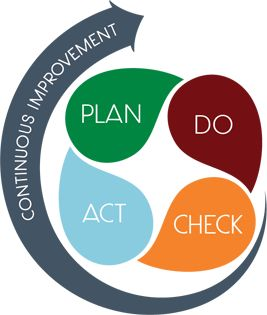
\includegraphics[scale=0.60]{Img/PDCA.jpg}
\caption{Attività del Principio di Deming}
\label{}
\end{figure}

\newpage
\section{CMM - Capability Maturity Model}
\label{app:CMM}
Il \gl{CMM}, acronimo di Capability Maturity Model, è un modello di sviluppo che ha lo scopo di migliorare i processi \gl{software} esistenti dal punto di vista dell'efficacia.
\newline Il nome del modello suggerisce i concetti su cui si basa:
\begin{itemize}
\item[-]\bold{Capability}: questa caratteristica indica la misura di quanto è adeguato un processo per gli scopi per cui è stato definito.
Determina pertanto l’intorno del risultato (di efficienza ed efficacia)
raggiungibile utilizzando quel determinato processo.
\newline Dunque un livello basso di tale caratteristica porterà alla produzione di esiti e di qualità scarsamente prevedibili, con un compromesso tra funzionalità e qualità. Al contrario avere un alto livello di Capability implicherà un uso sistematico, disciplinato e quantificabile del processo.
\item[-]\bold{Maturity}: questo termine si riferisce al grado di formalità e ottimizzazione dei processi, pertanto permette di misurare quanto sia governato il sistema dei processi all'interno di un'azienda.
\item[-]\bold{Model}: indica l'insieme di requisiti sempre più stringenti, che consentono di valutare il percorso di miglioramento dei processi di un’azienda.
\end{itemize}
\ 
\newline Tale modello fornisce:
\begin{itemize}
\item una base concettuale a cui far riferimento per valutare il livello dei processi;
\item un insieme di best practice consolidate negli anni da esperti e utilizzatori;
\item un linguaggio comune e una visione condivisa;
\item un metodo per definire un miglioramento in ambito organizzativo.
\end{itemize}

\subsection {Struttura}
Il modello \gl{CMM} presenta cinque aspetti che vanno a caratterizzare la sua struttura:
\begin{itemize}
\item \bold{Livelli di maturità} (Maturity levels): sono cinque livelli di maturità, dove il più alto (il quinto) è uno stato teoricamente ideale in cui i processi vengono sistematicamente gestiti attraverso una combinazione di ottimizzazioni di processi e miglioramenti continui di processi.
\\
\item \bold{Aree chiave di processo} (Key Process Areas): identifica un gruppo di attività correlate che, quando vengono eseguite insieme, producono una serie di obiettivi considerati strategici.
\\
\item \bold{Obiettivi} (Goals): gli obiettivi di un’area chiave di processo riassumono gli stati che devono esistere per quell’area per essere implementati in modo completo e duraturo. La quantità di obiettivi che sono stati raggiunti è un indicatore della Capability che l’organizzazione ha raggiunto in un certo livello di maturità.
\\
\item \bold{Caratteristiche comuni} (Common Features): le caratteristiche comuni includono le pratiche che sviluppano e regolamentano un’area chiave di processo. Ci sono cinque tipi di caratteristiche comuni: l’impegno nell’esecuzione, l’abilità nell’esecuzione, le attività eseguite, le misurazioni e le analisi, ed infine la verifica e l’implementazione.
\\
\item \bold{Pratiche fondamentali} (Key Practices): le pratiche fondamentali descrivono gli elementi dell’infrastruttura e le pratiche che contribuiscono in modo particolare all’implementazione e alla regolamentazione dell’area.
\end{itemize}

\subsection{Livelli di Maturity}
I livelli in cui è stata divisa la componente di Maturity del modello \gl{CMM} indicano il grado di maturità raggiunto dai processi; quanto più un processo rientrerà nei livelli alti tanto più sarà efficace, prevedibile e controllabile; per raggiungere tali livelli sarà necessario uno sviluppo incrementale da un livello a quello successivo (non è concesso saltare dei livelli).
\newline All'interno di ogni livello ci sono Aree chiave di processo che lo caratterizzano, e per ogni area ci sono a sua volta cinque fattori che la delineano: gli obiettivi, l'impegno, la capacità, la misurazione e la verifica.
\newline I cinque livelli sono i seguenti:
\\
\begin{enumerate}
\item \bold{Iniziale} (Initial)
\\I processi che rientrano in questo livello tipicamente risultano privi di ogni forma di documentazione e in uno stato di continuo cambiamento, riadattati ogni volta alle necessità del momento, poco riusabili ed incontrollati. Tutto questo porta ad un ambiente caotico e instabile per i processi.

\item \bold{Ripetibile} (Repeatable)
\\I processi di questo livello sono generalmente ripetibili, e spesso
danno buoni risultati; si inizia ad avere una certa disciplina nei processi che li porta ad essere rigorosi e robusti.

\item \bold{Definito} (Defined)
\\I processi iniziano ad essere raggruppati secondo standard definiti, vengono documentati e sono soggetti a miglioramenti nel lungo periodo. A questo livello gli standard di processo sono usati per consolidare l’esecuzione dei processi nell’organizzazione.

\item \bold{Gestito} (Managed)
\\A questo livello iniziano ad essere usate metriche di processo e i responsabili dell’azienda sono in grado di individuare i modi di adeguare e migliorare i processi rispetto a specifici progetti, senza rilevare perdite di qualità o deviazioni dalle specifiche.

\item \bold{Ottimizzante} (Optimizing)
\\I processi in questo livello sono volti a migliorare continuamente
le prestazioni attraverso cambiamenti e miglioramenti sia incrementali che tecnologicamente innovativi.
\end{enumerate}

\begin{figure}[htp]
\centering
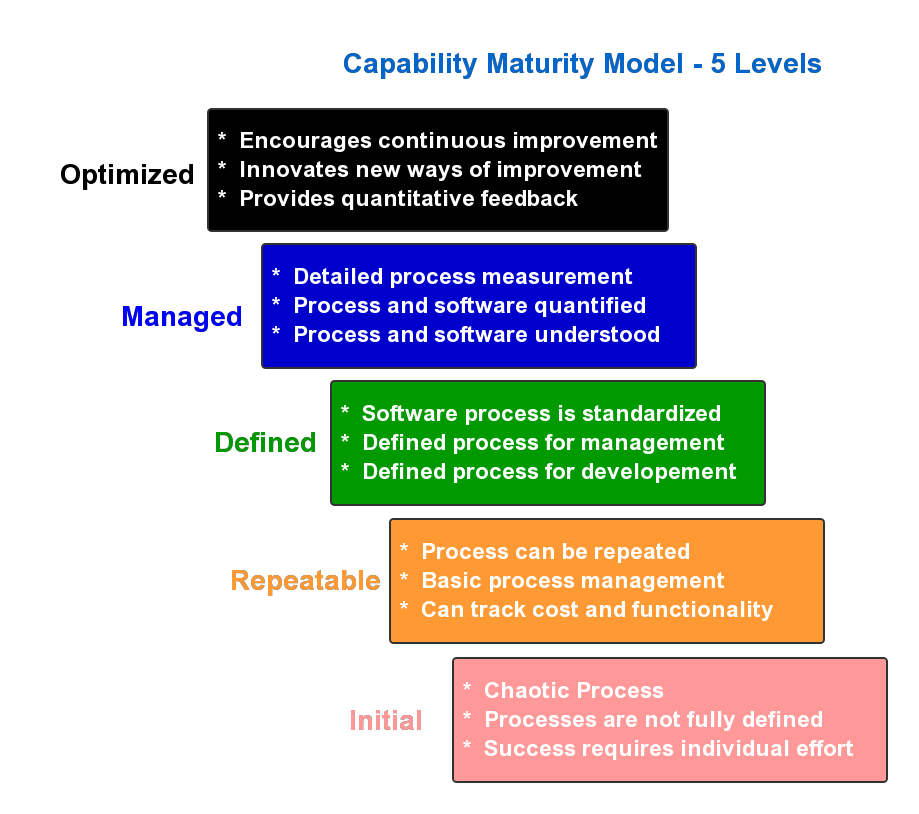
\includegraphics[scale=0.30]{Img/CMM.png}
\caption{Livelli di "Maturity" nel modello CMM}
\label{}
\end{figure}

\newpage
\section{ISO/IEC 9126}
\label{app:iso}
Le norme ISO/IEC 9126 descrivo un modello di qualità \gl{software}, definiscono le caratteristiche che la determinano e propongono metriche per la misurazione. 
\newline Le norme sono emesse dall'ISO, l'organismo internazionale di standardizzazione (International Organization for Standardization), cui aderiscono moltissimi paesi al mondo e collaborano diversi enti nazionali tra cui l'IEC, organo internazionale che definisce gli standard nel settore delle tecnologie dell'informazione e comunicazione (International Electrotechnical Commission).
\newline Il modello propone anche un approccio alla qualità affinché le società di \gl{software} possano migliorare l'organizzazione, i processi e a loro volta la qualità dei prodotti sviluppati.
\ 
\newline Le norme emesse dall'ISO/IEC 9126 suddividono i criteri qualitativi in tre macro aree:
\begin{itemize}
\item \bold{Qualità interna:} è la qualità del prodotto \gl{software} vista dall’interno e fa quindi riferimento alle caratteristiche implementative del \gl{software} quali l’architettura e il codice che ne deriva.
\item \bold{Qualità esterna:} è la qualità del prodotto \gl{software}  vista dall’esterno nel momento in cui esso viene eseguito e testato in un ambiente di prova.
\item \bold{Qualità in uso:} è la qualità del prodotto \gl{software} dal punto di vista dell’utilizzatore che ne fa uso all’interno di uno specifico sistema e contesto.
\end{itemize}
\ 
Basandosi sulle macro aree descritte le norme vengono divise nelle seguenti quattro parti:
\begin{enumerate}
\item Modello della qualità del \gl{software};
\item Metriche per la qualità esterna;
\item Metriche per la qualità interna;
\item Metriche per la qualità in uso.
\end{enumerate}

\subsection{Modello della qualità del software}
Lo standard inizialmente descrive il modello relativo alla qualità esterna e interna
e quello riguardante la qualità in uso.
\begin{figure}[htp]
\centering
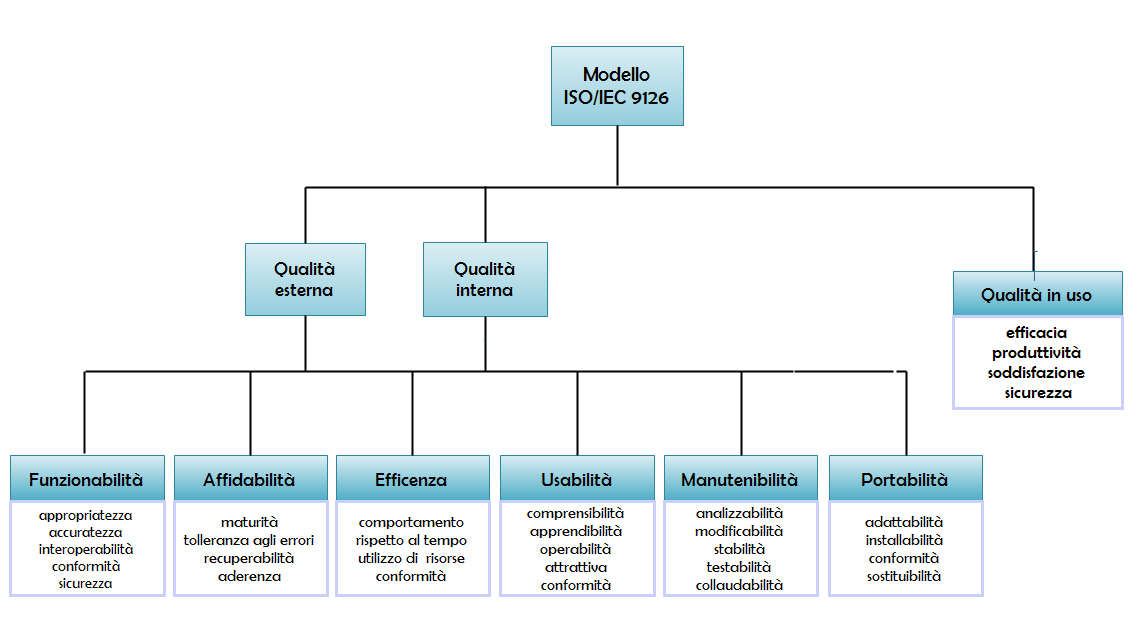
\includegraphics[scale=0.49]{Img/iso9126.png}
\caption{Modello della qualità del prodotto software secondo ISO/IEC 9126}
\end{figure}
\subsubsection{Modello della qualità interna ed esterna}
Sei caratteristiche identificano la qualità interna ed esterna del \gl{software} misurabili attraverso l'applicazione delle metriche presenti nello standard. Ogni caratteristica presenta a sua volta delle sottocaratteristiche che la specializzano.
\\
\begin{description}
\item \bold{Funzionalità}
\\ Questa caratteristica rappresenta la capacità del \gl{software} di fornire le funzioni, espresse ed implicite, necessarie per operare in un determinato contesto. 
\newline Le sottocaratteristiche che la compongono sono:
\begin{itemize}
\item[-]\bold{Adeguatezza:} capacità di fornire un appropriato insieme di funzioni che permettano agli utenti di svolgere determinati task per raggiungere gli obiettivi prefissati.
\item[-]\bold{Accuratezza:} capacità di fornire i risultati o gli effetti attesi con il livello di precisione richiesto.
\item[-]\bold{Interoperabilità:} capacità di interagire con uno o più sistemi specifici.
\item[-]\bold{Sicurezza:} capacità di proteggere le informazioni ed i dati in modo che persone non autorizzate non possano accedervi.
\item[-]\bold{Aderenza:} capacità di aderire agli standard, alle convenzioni e ai regolamenti che abbiano attinenza con la funzionalità.
\\
\end{itemize}

\item \bold{Affidabilità}
\\ Rappresenta la capacità di un prodotto \gl{software} di mantenere il livello di prestazione quando viene utilizzato in condizioni specifiche. Possibili limitazioni all'affidabilità possono esser causate da errori nei requisiti, nella progettazione oppure nel codice.
\newline Le sue sottocaratteristiche sono: 
\begin{itemize}
\item[-]\bold{Maturità:} capacità di evitare che si verifichino errori o siano prodotti risultati non corretti in fase di esecuzione.
\item[-]\bold{Tolleranza ai guasti:} capacità di mantenere il livello di prestazioni in caso di errori nel \gl{software}.
\item[-]\bold{Recuperabilità:} capacità di ripristinare il livello di prestazioni e di recuperare i dati direttamente coinvolti in caso di errori o malfunzionamenti.
\item[-]\bold{Aderenza:} capacità di aderire a standard, convenzioni e regole relative all'affidabilità.
\\
\end{itemize}
\item \bold{Usabilità}
\\ Questa caratteristica rappresenta la capacità di un prodotto \gl{software} di essere comprensibile, di poter essere studiato e di risultare attraente per un utente finale sotto determinate condizioni.
Alcuni aspetti di funzionalità, efficacia e affidabilità vanno a incidere su questa caratteristica.
\newline Le sue sottocaratteristiche sono:
\begin{itemize}
\item[-]\bold{Comprensibilità:} capacità di permettere all'utente di capire la sua funzionalità e come poterla utilizzare con successo.
\item[-]\bold{Apprendibilità:} capacità di permettere all'utente finale di imparare ad usare l'applicazione.
\item[-]\bold{Operabilità:} capacità di permettere all'utente di utilizzare e controllare il prodotto
\item[-]\bold{Attrattività:} capacità di risultare attraente per l'utente finale, in riferimento all'aspetto grafico.
\item[-]\bold{Aderenza all'usabilità:} capacità di aderire a standard, convenzioni, stili e regole relative all'usabilità.
\\
\end{itemize}

\item \bold{Efficienza}
\\È la capacità per un prodotto \gl{software} di realizzare, in determinate condizioni, le funzioni richieste nel minor tempo possibile attraverso l'uso migliore delle risorse necessarie.
\newline Le sottocaratteristiche che la compongono sono:
\begin{itemize}
\item[-]\bold{Comportamento rispetto al tempo:} capacità di fornire appropriati tempi di risposta, tempi di elaborazione, e quantità di lavoro eseguendo le funzionalità previste.
\item[-]\bold{Utilizzo delle risorse:} capacità di utilizzare un appropriato numero e tipo di risorse (umane e non) quando si eseguono le funzionalità previste sotto determinate condizioni di utilizzo.
\item[-]\bold{Aderenza all'efficienza:} capacità di aderire a standard e convenzioni relative all'efficienza.
\\
\end{itemize}
\item \bold{Manutenibilità}
\\Per un prodotto \gl{software} tale caratteristica rappresenta la capacità di essere modificato attraverso correzioni o adattamenti rispetto a modifiche negli ambienti, nei requisiti e nelle specifiche funzionali.
\newline Le sue sottocaratteristiche sono:
\begin{itemize}
\item[-]\bold{Analizzabilità:} capacità di poter effettuare la diagnosi sul \gl{software} ed individuare le cause di errore e/o malfunzionamento.
\item[-]\bold{Modificabilità:} capacità di consentire lo sviluppo di modifiche al \gl{software} originale. L'implementazione include modifiche al codice, alla progettazione e alla documentazione.
\item[-]\bold{Stabilità:} capacità di evitare effetti non desiderati a seguito di modifiche al \gl{software}.
\item[-]\bold{Provabilità:} capacità di consentire la verifica e la validazione del \gl{software} modificato (possibilità di esecuzione dei test).
\item[-]\bold{Aderenza alla manutenibilità:} capacità di aderire a standard e convenzioni relative alla manutenibilità.
\\
\end{itemize}

\item \bold{Portabilità}
\\ Rappresenta la capacità per un prodotto \gl{software} di poter essere trasportato da un ambiente (\gl{software}/\gl{hardware}) ad un altro.
\newline È identificato dalle seguenti sottocaratteristiche:
\begin{itemize}
\item[-]\bold{Adattabilità:} capacità di essere adattato a differenti ambienti senza richiedere azioni specifiche diverse da quelle previste dal \gl{software} per tali attività.
\item[-]\bold{Installabilità:} capacità di essere installato in un determinato ambiente.
\item[-]\bold{Coesistenza:} capacità di coesistere con altre applicazioni indipendenti in ambienti comuni e con risorse condivise.
\item[-]\bold{Sostituibilità:} capacità di sostituire un altro \gl{software} specifico indipendente, per lo stesso scopo e nello stesso ambiente.
\item[-]\bold{Aderenza alla portabilità:} capacità di aderire a standard e convenzioni relative alla portabilità.
\end{itemize}
\end{description}

\subsubsection{Modello della qualità in uso}
La qualità in uso rappresenta il punto di vista dell'utente finale sulla qualità; tale qualità viene raggiunta qualora siano precedentemente raggiunti i livelli di qualità interna ed esterna.
\newline Gli attributi della qualità in uso sono rappresentati dalle seguenti macro categorie:
\begin{description}
\item \bold{Efficacia}
\\ Rappresenta la capacità per un prodotto \gl{software} di premettere all'utente di raggiungere obiettivi specifici con accuratezza e completezza in uno specifico contesto di utilizzo.
\item \bold{Produttività}
\\Rappresenta la capacità di permettere all'utente di impegnare un numero definito di risorse, in relazione all'efficacia raggiunta in uno specifico contesto di utilizzo.
\item \bold{Sicurezza fisica} 
\\ Identifica la capacità di raggiungere un livello accettabile di rischio per i dati, le persone, il business, la proprietà o gli ambienti in uno specifico contesto di utilizzo.
\item \bold{Soddisfazione}
\\ Rappresenta la capacità di soddisfare gli utenti in uno specifico contesto di utilizzo, in riferimento alle iterazioni dell'utente con il prodotto finale.
\end{description}

\subsection{Metriche per la qualità interna}
Le metriche interne vengono applicate al \gl{software} non eseguibile (specifiche tecniche e codice sorgente) durante le fasi di progettazione e codifica, oltre che alla documentazione. Pertanto durante le fasi di sviluppo del \gl{software} i prodotti intermedi vengono valutati tramite tali metriche interne che possano misurare le proprietà intrinseche del prodotto.
\newline Le metriche interne permettono ad utenti, verificatori e sviluppatori di segnalare per tempo eventuali problemi che potrebbero inibire la qualità finale del prodotto.

\subsection{Metriche per la qualità esterna}
Le metriche esterne misurano i comportamenti del prodotto \gl{software} rilevabili dai test, dall'operatività, dall'osservazione durante la sua esecuzione. L’esecuzione del prodotto \gl{software} è fatta in un contesto tecnico rilevante.
\newline Le metriche esterne sono scelte in base alle caratteristiche che il prodotto finale dovrà dimostrare durante la sua esecuzione in esercizio.

\subsection{Metriche per la qualità in uso}
Le metriche per la qualità in uso misurano invece il grado con cui il prodotto \gl{software} permette agli utenti di svolgere le proprie attività con efficacia, produttività, sicurezza e soddisfazione nel contesto operativo previsto. Per questo la valutazione della qualità finale del prodotto \gl{software} dev'essere fatta in specifici scenari d'uso.

\newpage
\section{Attività di Analisi requisiti utente \\\large{resoconto~delle~sottoattività~di~verifica}}
\label{app:valtest}

\subsection{Verifica dei processi}
\subsubsection{Documentazione}
\myparagraph{Schedule Variance}
Vengono riportati di seguito i valori ottenuti calcolando la Schedule Variance sui tempi di stesura di ogni documento:
\begin{tabella}{l!{\VRule}c!{\VRule}c!{\VRule}}
	\color{white} \bold{Documento} & \color{white} \bold{SV in giorni} &\color{white} \bold{Giudizio} \\
	\endfirsthead
	Analisi dei Requisiti v1.0 & +2 & Accettabile \\
	Norme di Progetto v1.0 & 0 & Ottimale \\
    Studio di Fattibilità v1.0 &  -1 &  Ottimale \\
    Piano di Progetto v1.0 &  0 &  Ottimale\\
    Piano di Qualifica v1.0 & -2 & Ottimale \\
    Glossario v1.0 & +2 & Accettabile\\	
	\rowcolor{white}  
	\caption{Esiti della Schedule Variance - Attività di Analisi requisiti utente}	    	
\end{tabella}

\bold{Considerazioni finali:}
\begin{description}
\item{\bold{Schedule Variance finale:}} +1 giorno.
\\In generale per il processo di documentazione il \gl{team} ha ritardato la stesura di 1 giorno rispetto a quanto pianificato nel \doc{Piano di Progetto}. Il risultato ottenuto pertanto rientra nella soglia di accettabilità prevista.
\end{description}


\myparagraph{Cost Variance}
Vengono riportati di seguito i valori ottenuti calcolando la Cost Variance sui tempi di stesura di ogni documento:
\begin{tabella}{l!{\VRule}c!{\VRule}c!{\VRule}}
	
	\color{white} \bold{Processo} & \color{white} \bold{CV} &\color{white} \bold{Giudizio} \\
	\endfirsthead
	Processo di documentazione & 0\% & Ottimale\\
	\rowcolor{white}  
	\caption{Esiti della Cost Variance - Attività di Analisi requisiti utente}	   	
\end{tabella}

\bold{Considerazioni finali:} Per il processo di documentazione il \gl{team} non ha necessitato di ulteriori risorse che potessero aumentare i costi pianificati precedentemente.

\newpage
\myparagraph{Capability Maturity Model}
Si è cercato di valutare la qualità del processo di documentazione secondo le metriche stabilite dal modello \gl{CMM} . Ovviamente, quando il progetto è cominciato si era al livello 1 dei livelli di Maturity: le procedure e le norme erano completamente informali, non era presente alcun tipo di documentazione e lo stato risultava caotico, non permettendo alcun tipo di ripetibilità di procedure in modo certo.
\newline In seguito alla redazione del documento \NdPdoc sono state definite  norme valide per ogni tipo di documentazione, strumenti comuni
da poter utilizzare e procedure da seguire per effettuare determinate attività. Il processo di documentazione ha in questo modo guadagnato ripetibilità come viene richiesto al livello 2 del modello \gl{CMM}.
\newline La soglia di accettabilità, descritta nella sezione \hyperref[sec:metr]{Misure e metriche}, pertanto è stata raggiunta per tale processo, ma ciò che è stato fatto non è sufficiente per raggiungere anche il livello 3.
\newline Nelle prossime attività si cercherà di apportare un incremento di qualità al processo di documentazione.

\subsubsection{Verificazione}
\myparagraph{Schedule Variance}
Vengono riportati di seguito i valori ottenuti calcolando la Schedule Variance sui tempi di stesura di ogni documento:
\begin{tabella}{l!{\VRule}c!{\VRule}c!{\VRule}}
	
	\color{white} \bold{Documento} & \color{white} \bold{SV in giorni} &\color{white} \bold{Giudizio} \\
	\endfirsthead
	Analisi dei Requisiti v1.0 & +2 & Accettabile \\
	Norme di Progetto v1.0 & -1 & Ottimale \\
    Studio di Fattibilità v1.0 &  0 &  Ottimale \\
    Piano di Progetto v1.0 &  0 &  Ottimale\\
    Piano di Qualifica v1.0 & -1 & Ottimale \\
    Glossario v1.0 & 0 & Ottimale\\	
	\rowcolor{white}  
	\caption{Esiti della Schedule Variance - Attività di Analisi requisiti utente}	    	
\end{tabella}

\bold{Considerazioni finali:}
\begin{description}
\item{\bold{Schedule Variance finale:}} 0 giorni.
\\Per il processo di verificazione, in generale, il \gl{team} ha ritardato di 0 giorni rispetto a quanto pianificato nel \doc{Piano di Progetto}. Pur essendoci documenti che sono stati verificati in ritardo, il valore generale ottenuto rientra nella soglia di accettabilità prevista.
\end{description}
\newpage
\myparagraph{Cost Variance}
Vengono riportati di seguito i valori ottenuti calcolando la Cost Variance sui tempi impiegati nel processo di verificazione:
\begin{tabella}{l!{\VRule}c!{\VRule}c!{\VRule}}
	
	\color{white} \bold{Processo} & \color{white} \bold{CV} &\color{white} \bold{Giudizio} \\
	\endfirsthead
	Processo di verifica & 0\% & Ottimale\\
	\rowcolor{white}  
	\caption{Esiti della Cost Variance - Attività di Analisi requisiti utente}	  
\end{tabella}

\bold{Considerazioni finali:} Per il processo di verificazione il \gl{team} non ha necessitato di ulteriori risorse che potessero aumentare i costi pianificati precedentemente.

\myparagraph{Capability Maturity Model}
Il processo di verificazione è da considerarsi uno dei più importanti poiché deve risultare efficiente ed efficace per tutta la durata del progetto, dal momento che dev'essere eseguito molteplici volte ed ha un costo elevato.
\newline Come per il processo di documentazione, anche per quello di verificazione si è partiti dal livello 1 della classificazione di Maturity presente nel modello \gl{CMM}. Il modo di procedere era caotico e non ripetibile, attraverso l'individuazione di strumenti e tecniche per eseguire il processo di verifica è stato possibile renderlo più disciplinato, controllato e ripetibile (anche attraverso l'uso di strumenti automatici).
\newline Si è pertanto raggiunto il livello 2 (Ripetibile) come ci si attendeva, rispettando la soglia di accettabilità, descritta nella sezione \hyperref[sec:metr]{Misure e metriche}.

\subsection{Verifica dei prodotti}
\subsubsection{Documenti}
\myparagraph{Errori ortografici}
Il gruppo, attraverso un processo di verifica automatica e manuale, ha individuato parecchi errori di battitura all'interno dei documenti.
\newline Vengono riportati di seguito i valori ottenuti riguardanti la verifica degli errori ortografici:
\begin{tabella}{l!{\VRule}c!{\VRule}c!{\VRule}}
	
	\color{white} \bold{Documento} & \color{white} \bold{Errori ortografici} &\color{white} \bold{Giudizio} \\
	\endfirsthead
	Analisi dei Requisiti v1.0 & 2\% & Accettabile\\
	Norme di Progetto v1.0 & 1\% & Accettabile\\
    Studio di Fattibilità v1.0 & 2\% &  Accettabile \\
    Piano di Progetto v1.0 & 2\% & Accettabile \\
    Piano di Qualifica v1.0 & 3\% & Accettabile\\
    Glossario v1.0 & 1\% & Accettabile\\	
	\rowcolor{white}  
	\caption{Esiti degli Errori Ortografici - Attività di Analisi requisiti utente}	    	
\end{tabella}

\bold{Considerazioni finali:}
Per ogni documento il \gl{team} ha svolto un buon lavoro nella correzione degli errori ortografici, anche se non tutti sono stati corretti subito. In ogni caso la percentuale di errori individuati in ogni documento rientra nella soglia di accettabilità prevista dalla metrica.

\newpage
\myparagraph{Indice Gulpease}
Ogni documento è stato sottoposto ad uno \gl{script} che ne calcolasse l'\gl{Indice Gulpease} per valutarne il grado di leggibilità.
\newline Di seguito vengono presentati i dati raccolti:
\begin{tabella}{l!{\VRule}c!{\VRule}c!{\VRule}}
	
	\color{white} \bold{Documento} & \color{white} \bold{\gl{Indice Gulpease}} &\color{white} \bold{Giudizio} \\
	\endfirsthead
	Analisi dei Requisiti v1.0 &  51 & Accettabile \\
	Norme di Progetto v1.0 & 53 & Accettabile\\
    Studio di Fattibilità v1.0 & 59 & Accettabile \\
    Piano di Progetto v1.0 & 49 & Accettabile \\
    Piano di Qualifica v1.0 & 45 & Accettabile\\
    Glossario v1.0 & 59 & Accettabile\\	
	\rowcolor{white}  
	\caption{Esiti dell'\gl{Indice Gulpease} - Attività di Analisi requisiti utente}	    	
\end{tabella}
\bold{Considerazioni finali:}
Dai risultati ottenuti è possibile stabilire che ogni documento presenta un buon grado di leggibilità. Ogni valore rientra appieno nella soglia di accettabilità indicata da tale metrica.

\myparagraph{Errori Concettuali}
Il gruppo ha posto molta attenzione nell'uso di termini, concetti teorici e contenuti più generali in modo da non cadere in contraddizioni, nell'uso di terminologie sbagliate o di concetti teorici errati. Durante il processo di verificazione dei documenti pertanto non è stato riscontrato nessun tipo di errore concettuale a cui sia stato necessario apportarne una modifica. 
\newline La soglia di accettabilità in tal modo viene rispettata e addirittura viene raggiunto il valore ottimale per tale metrica, descritta nella  sezione \hyperref[sec:metr]{Misure e metriche}.

\myparagraph{Errori di forma}
Sono stati segnalati, dai \italics{Verificatori}, diversi errori di forma che non rispettavano le norme descritte nel documento \italics{Norme di Progetto}. La maggior parte sono stati corretti, ma una minima parte è sfuggita durante l'azione di correzione e pertanto sono stati segnalati durante una nuova azione di verifica.
\newline In ogni caso la percentuale di errori di forma, per come è descritta tale metrica nella sezione \hyperref[sec:metr]{Misure e metriche}, risulta pari all'1\%; valore che rientra pienamente all'interno della soglia di accettabilità prevista.
\newpage
\subsection {Sommario del resoconto delle sottoattività di verifica}

\begin{tabella}{l!{\VRule}>{\centering\arraybackslash}p{6 cm}!{\VRule}>{\centering\arraybackslash}p{2 cm}!{\VRule}>{\centering\arraybackslash}p{2 cm}}

		
	
	\color{white} \bold{Verifica} & \color{white} \bold{Metrica} & \color{white} \bold{Giudizio finale} \\
	\endfirsthead
	
	\cellcolor{P} & Schedule Variance & Accettabile\\
	\cellcolor{P} & Cost Variance & Ottimale \\
	\multirow{-3}{*}{\cellcolor{P}Processo di Documentazione}	& Capability Maturity Model & Accettabile \\
	\hline
	
	\cellcolor{D} & Schedule Variance & Accettabile \\
	\cellcolor{D} & Cost Variance & Ottimale \\
	\multirow{-2}{*}{\cellcolor{D}Processo di Verificazione} & Capability Maturity Model & Accettabile \\
	\hline
	
	\cellcolor{P} & Errori Ortografici & Accettabile \\
	\cellcolor{P} & \gl{Indice Gulpease} & Accettabile \\
	\multirow{-2}{*}{\cellcolor{P} Documenti} & Errori Concettuali & Ottimale \\ & Errori di Forma & Accettabile \\
	\hline
		

	\caption{Riassunto del Resoconto delle sottoattività di verifica - Attività di Analisi requisiti utente}	    	
	
\end{tabella}




\end{document}